%\renewcommand{\tabularxcolumn}[1]{m{#1}}
%\newcolumntype{Y}{>{\centering\arraybackslash}X}
%\newcolumntype{R}{>{\flushright\arraybackslash}X}



\renewcommand{\thesection}{\arabic{chapter}.\arabic{section}}



\chapter{Dynamics of the Electricity Day-Ahead Market : Supply Function Equilibria and Ramping Costs}
\label{chap:ch1}
\cleardoublepage

%\doublespacing
\section{Introduction}
\subsection{Litterature review}
The electricity markets have flourished in Europe during the 1990s during the wave of privatisation. The argument for their creation was one of competition, that was supposed to bring lower prices to the end consumer of electricity.\\

An important specificity to the economics of electricity is that electricity cannot be stored in large amounts, which in turn implies that at every moment production and consumption have to match. This means that in order to have a working electric grid, that is one that can produce electricity for high levels during the winter and lower levels in summer, one has to have production units ready to be turned on if the demand is high enough, but turned off otherwise. This in turn means that although their existence is required, it is difficult to see how to marginal cost pricing can cover their investment costs, which has been a long running argument in the litterature \cite{boiteux1960peak}. For this reason, from the very beginning the issue of the market design was deemed to be crucial to insure that the wished for outcome of the privatization wave came to fruition \cite{green1991reshaping}. \\

Most countries having open the production of electricity to competition have implemented day-ahead markets. As said above, the production and the consumption have to match constantly. The very short term matching is done by automating tiny adjustments around what a producer is already producing in order to match the fluctuating consumption. To plan which plant should be online at which hour of the day however, the day-ahead markets come in. The idea is that producers and big consumers of electricity (either for themselves, or as aggregators of the individual consumptions) are asked to bid demand or supply functions respectively. The market operator then aggregates the demand and supply curves, which yields an equilibrium giving the price and quantities to be produced for each producer.  \\

There has been an active litterature trying to model and measure the market power of oligopolists on these newly created markets \cite{Newgreen, newbery1998competition, green1999electricity}. The models have mainly been based on Klemperer and Meyer 1989's Econometrica founding paper about supply function equilibria \cite{KM} (henceforth known as KM). 

This paper builds upon previous results about competition in supply schedules without uncertainty \cite{grossman1981nash}, which yielded a very high multiplicity of equilibria. KM add a key ingredient : uncertainty about the demand schedule facing the suppliers. This addition reduces greatly the multiplicity, and adds more structure to it, although in this framework there is still a continuum of Nash equilibria, which are always pinned between Cournot and Bertrand outcomes. \\

Groundbreaking and fertile, the original model by KM studied how demand uncertainty collapses dramatically the set of available supply function equilibria to a well defined continuum when contrasted to the case of competition in supply schedules without uncertainty \cite{grossman1981nash}. These equilibria are always pinned between Cournot and Bertrand outcomes. This continuum collapses further to a single Nash equilibria by considering an infinite support of demand shocks. All of these equilibria are ex-post optimal, meaning that changes in anticipated demand shocks do not impact the actual solutions, but only the parts of the solutions that are actually explored as shocks realize. In this setup markets are always efficient, a very strong result. \\

The electricity markets litterature has embraced this framework because it is considered to capture some of the structure at play in the electricity markets : the producers do not know what demand they are going to face when they choose their supply schedule, the demand side is considered much less sophisticated than the supply side, and their demand schedules can therefore be considered to some extent as being exogenous. Some have argued that the schedules submitted in the real markets are discrete and that this discrete nature makes their modelling as continuously differentiable schedules is both incorrect and yields different results from discrete ones \cite{von1993spot}. However recent results suggest that with a sufficient amount of steps both approaches converge \cite{holmberg2008supply}, and indeed we see that recent implementations of the market rules increase the number of steps allowed for a single bid, and consider that these points are linearly joined instead of stepwise.\\

One of the mose striking aspects of the supply function equilibria approaches is, as was alluded to above, the multiplicity of Nash equilibria. This result has been generally viewed as the source of the danger of tacit collusion in electricity markets : if there is a continuum of nash equilibria, repeated interactions are feared to be conducive to a convergence of bidding strategies towards the most profitable equilbria \cite{bolle1992supply}. \\

Furthermore, these models abstract away some of the details of the actual markets, reason for which authors which try and evaluate the market power of producers on the electricity markets view their endeavour as painting the situation with an optimistic brush \cite{Newgreen}. \\

Here we will tackle the points raised in the last two paragraphs to some extent. We propose to consider a technical reality of the operating of power plants : their cost structure is history-dependant, more precisely, producing a quantity $q1$ does not entail the same cost if the previous quantity produced was already $q_1$ or if the previous quantity was different from it. Raising or decreasing production in and of itslef imply costs. By introducing these costs we aim to produce a model capable of capturing more precisely the competition that arises in the electricity markets, and in so doing we will show that the continuum of equilibria caracteristic of supply function equilibria under uncertainty collapses to unique equilibria, which in turn allows us to comment on the question of tacit collusion.\\


%
%One traditional understanding for the role of markets is that a market allows to aggregate information that would be otherwise dispersed. When applying this view to the electricity markets, the litterature has regarded the existence of the capacity market as a way to aggregate information about investment costs when building a plant, the existence of the forward market as a way to aggregate information about the fixed costs, and the existence of the spot market as a way to aggregate information about marginal costs. \\
%
%
%At the same time, the litterature as well as the industry is well aware of the existence of ramping costs, that is costs that depend on the variation of production. We think that the two spot markets can be understood as aggregating information about marginal costs and ramping costs. In this paper we model the day-ahead market using the supply function equilibria framework and considering that there exists ramping costs. This allows us to obtain unique solutions, in contrast to the usual continuum, and to describe the dynamic evolution of the optimal bid in a symmetric oligopoly. It also opens the possibility to distinguish between day-ahead and intraday markets. \\
%
%%However, the spot market is actually divided into two markets : the day-ahead market and the intraday or balancing market, that the litterature does not differentiate clearly.
%
%The supply function equilibria litterature has been active since the seminal paper by Klemperer and Meyer in 1989 \cite{KM} (henceforth known as KM). In the wake of the electricity industry liberalisation, authors, notably Green and Newbery in 1992 \cite{Newgreen}, have used this framework to evaluate the expected level of competition and argue for certain regulatory paths. \\

\subsection{The day-ahead markets}

On the electricity day ahead markets, producers are generally required to submit supply schedules once a day for all the auctions taking place during the next day. The APX (England) and the EPEX (Austria, France, Germany and Switzerland) markets allow hourly auctions \cite{apx,epex}, and EPEX allows for bids comprising up to $256$ price quantity combinations, effectively approximating smooth supply functions. Producers can submit different supply schedules for each individual auction, but every bid must be placed at the same time one day in advance for each block of 24 hours. Customers go through the same process and submit their demand schedules, then the market operator matches supply and demand for each auction. Producers thus have to submit schedules facing uncertain demand, this is the reason for the popularity of supply function equilibria approaches to the electricity market.\\   

However, on this market, bids change from auction to auction. From the point of view of KM's model, this should happen only through a coordination of agents agreeing to collectively swap from one Nash equilibrium to another in the available continuum. Describing these dynamics, however, is increasingly important as the energetic mix is bound to include an increasing fraction of renewables. Power production can be separated in two classes: dispatchable and non-dispatchable technologies. Nuclear, coal, land-fill gas or hydroelectric power generation are mainly dispatchable as one can actually choose their level of production whereas the two rising stars of renewable energy, namely wind and solar, are non-dispatchable: they react to weather conditions. Having these technologies in the mix introduces uncertainty on the production side, which comes down to dispatchable units facing a more uncertain residual demand \cite{Boyle}. In this paper we want to explore how to model these dynamics. \\

Electricity production faces very specific technological constraints. These constraints, generally labelled as ramping costs, vary across production technologies, and have yet to be captured in a model. We propose to do so by introducing a multivariate cost function, depending as always on the quantity produced, but also on the rate at which production varies: $C(S,\frac{dS}{dt})$. We call this class of cost functions dynamic cost functions.\\

All power plants face maintenance costs. However part of these maintenance costs are induced by the dynamics of production, and can be seen as ramping costs. More precisely, whatever the production technology, fluctuations in production are costly. Indeed, they imply fluctuations in the temperature of the core of the power plant, thus dilation and contraction cycles of the different parts, which cause wear and tear. The industry is aware of these effects \cite{GE}, some B2B companies even specialize in minimizing the related long term costs. For example, Wartsila Power Plants, a supplier of power plants and tools to forecast long term costs, explains in a white paper \cite{Arima}: 
\begin{quote}
Increased variability in net load demand means that dispatchable generating units have to ramp considerably more steeply and deeper than traditionally, thus increasing wear and tear to components.
\end{quote}
We are going to model these ramping costs through a dynamic cost function, increasing in the absolute value of its second argument : any change in production is costly. This paper will focus on the implications of considering this type of ramping costs. Other types of ramping costs exist, for example startup costs, but they will not be studied in this paper. \\

These effects cannot be captured by traditionnal cost functions depending on the level of production alone. One needs to take into account the actual path leading to a given quantity produced. This implies that we need to impose structure on the dynamics of the system while retaining uncertainty, the key ingredient of KM's paper. To do so, we use stochastic dynamics. \\

This seemingly small addition to KM's framework has a lot of implications on the results obtained. The solutions are not ex-post optimal anymore, allowing to account more satisfactorily for the dynamics of optimal supply schedules, and our solutions are unique, even for bounded demand shocks. We also define a novel selection rule to choose from KM's continuum of equilibria. Finally these results open the possibility to distinguish intraday and day-ahead markets. \\ 

%In section \ref{litrev} we will present how this paper contributes to the litterature, i
In section \ref{heur} we will present a heuristic approach to get the intuition of the model. Then, in section \ref{math} we will introduce the mathematical tools needed to use stochastic dynamics in this context, in section \ref{monosolve} and section \ref{oligosolve} we will solve the monopoly and the symmetric oligopoly cases while considering that producers have information about the overall distribution of shocks during the day, but do not have information about differences in the shocks at different dates. Finally in section \ref{dynamics} we will discuss the dynamic variation of the optimal bids, while sections \ref{disc} and \ref{ccl} will respectively cover a few implications of these results and conclude the paper.  

%\section{Litterature Review}\label{litrev}
%TO BE FILLED
\section{Heuristic Description of the Model}\label{heur}
In this section the essence of the model is presented before introducing the proper mathematical tools needed to treat this problem rigorously in the next section. \\

As in KM's setup, the producer faces uncertain demand, $D(\theta,p)$, with $\theta$ a stochastic shock to the demand and $p$ the price, to which we add ramping costs and uncertain dynamics of demand: $\theta(t)$ is the time trajectory of a stochastic shock with stochastic dynamics. In the real market, bidders submit a finite number of bids once a day, and face the ramping costs inter-period, that is, when production has to be adjusted to reach the subsequent market outcome. Here we assume that time is continuous, that ramping costs are incurred continuously, and that bidders are allowed to submit a different supply schedule for every point in time. This amounts to being asked to submit a surface of strategy in the price-quantity-time space. \\

The producer maximises her expected profits, and we consider here the simplest case in which the distribution of shocks is static and the producer is asked by the market operator to submit a single supply schedule a day in advance. In an oligopoly the program maximised by producer $i$ is therefore:

\begin{equation}
\displaystyle{\max_{S_i(p)}}~\mathbb{E}\left[\int_{0}^{T} \left(p(\theta(t))S_i(p(\theta(t))) -C\left(S_i(p(\theta(t))),\frac{dS_i(p(\theta(t)))}{dt} \right)\right)dt\right]
\end{equation}
with $p(\theta(t))$ the price given the demand shock $\theta(t)$ at date $t$, $S_i(\cdot)$ the supply schedule of producer $i$ and $C(\cdot,\cdot)$ the dynamic cost function.  \\

The goal of this section is to provide the intuition of the model, therefore we will not describe here the conditions that must be verified by the different terms of the model. We will simply assume that the dynamic cost function is additively separable between a static and a ramping term, $C(S_i,\frac{dS_i}{dt})=C_s(S_i)+C_r(\frac{dS_i}{dt})$, and that the demand shocks $\theta$ are bounded in $[\underline{\theta},\overline{\theta}]$. Lastly we require the ramping term $C_d(\cdot)=\frac{\gamma}{2}(\cdot)^k$ for clarity, and $k\geq2$ an integer. We distribute the expectation operator and write that $\frac{dS_i}{dt}=\frac{dS_i}{dp}\frac{dp}{d\theta}\frac{d\theta}{dt}=S_i'\cdot \dot{p}\cdot \frac{d\theta}{dt}$, with $X'$ the derivative of univariate function $X$ with respect to its argument, $\dot{X}=\frac{dX}{d\theta}$. The maximisation program can then be written as follows :
\begin{equation}
\displaystyle{\max_{S_i(p)}}~\int_{\underline{\theta}}^{\overline{\theta}} f(\theta)\left(p(\theta)S_i(p(\theta(t))) -C_s(S_i(p(\theta(t))))-\frac{\gamma}{2}\left(S_i'\cdot\dot{p}\right)^k\mathbb{E}\left[\left(\frac{d\theta}{dt}\right)^k\middle \vert \theta  \right]\right)d\theta
\label{maxbase}
\end{equation}
with $f(\theta)$ the distribution of shocks, and $\gamma$ the ramping cost parameter capturing the magnitude of the ramping costs.\\

Note that $\mathbb{E}\left[\left(\frac{d\theta}{dt}\right)^k\middle \vert \theta  \right]$ depends only on $\theta$, and that producer $i$ faces a residual demand so that $S_i(p(\theta(t)))=D(\theta,p(\theta(t)))-S_{-i}(p(\theta(t)))$ which depends only on $\theta$ and $p$, with $S_{-i}$ the aggregate supply schedule of all the other producers, taken as given by producer $i$. This implies that the integrand in eq. \ref{maxbase} depends only on three variables: $\theta$, $p$ and $\dot{p}$.  The maximisation pogram is therefore equivalent to an Euler-Lagrange problem, a very well described mathematical object: $\max_p\int\mathcal{L}(\theta,p,\dot{p})d\theta$. \\

The information obtained from taking the first-order condition of an Euler-Lagrange problem yields a second order differential equation as well as two boundary conditions: $\frac{\partial\mathcal{L}}{\partial p}=\frac{d}{d\theta}\frac{\partial\mathcal{L}}{\partial \dot{p}}$ and $\frac{\partial\mathcal{L}}{\partial\dot{p}}\big|_{\underline{\theta}}=\frac{\partial\mathcal{L}}{\partial\dot{p}}\big|_{\overline{\theta}}=0$. This is why we obtain unique solutions: if the boundary conditions are not verified there exists profitable deviations. In less mathematical terms, taking ramping costs into account as specified above means that for a given level of shock, one not only cares about the optimal level of production for this shock, but also about the optimal slope of the supply schedule at this level of production. Effectively, this means that optimal levels of production cannot be chosen independently for different level of shocks anymore, thus shrinking the continuum of equilibria. The boundary conditions' argument explains why the continuum not only shrinks, but collapses to a unique equilibrium. \\

Note that if the ramping cost parameter $\gamma$ is taken equal to $0$ we are back to KM's model: one doesn't care about the slope of the supply schedule anymore, and the problem comes down to a pointwise maximisation which therefore yields ex-post optimal equilibria. We want to stress that this means that it is not sufficient to specify the dynamics of the shocks to obtain a dynamic model, one needs to take into account ramping costs.\\

The maximisation program~\ref{maxbase} is a heuristic description of the situation. We want to model the stochastic nature of demand and of its dynamics. We do this by using It\={o} processes, a class of stochastic processes built through brownians, to describe the stochastic trajectory of the demand shocks with respect to time. The difficulty is that brownians are everywhere continuous but nowhere differentiable, therefore the way program~\ref{maxbase} is written, with a term in $\frac{d\theta}{dt}$, is incorrect.\\

In the next section we introduce the stochastic dynamics properly without using the concept of derivative. 


\section{Stochastic Dynamics}\label{math}

As described in the previous section, we consider that bidders submit surfaces, that is supply schedules for every point in time. The reason to describe a discrete dynamic market as a continuous one is that although discrete time is conceptually more easily understood, continuous time allows to use much more powerful mathematical tools and to obtain closed form solutions, which we think are crucial in gaining intuitive insights about these dynamics. Therefore we consider that demand fluctuates continuously and that ramping costs are incurred instantaneously. This approximation would need to be tested, although it should be noted that day ahead markets operate with hourly or half-hourly periods and are therefore facing a reasonnable amount of periods each day. \\ 

Our strategy to describe a discrete process as a continuous one is as follows. We approximate the stochastic process (continuous in time) that we want to use to describe the market by a random walk (discrete in time), and then decrease its timescale towards $0$ to converge towards the stochastic process. We are first going to describe the target stochastic process that we will be using throughout this paper, before illustrating how we go from a discrete description to a continuous one. \\

In the electricity market, demand shocks, denoted $\theta(t)$, are bounded: there are no days for which demand is null nor are there days for which demand tends towards infinity. The structure to be imposed on the dynamics of the shocks has to imply bounded shocks. \\

\subsection{The stochastic process}
A simple It\={o} process one can consider that leads to bounded shocks is defined by the following stochastic differential equation (SDE):
\begin{equation}
d\theta(t)=-2\theta(t) dt+\sqrt{1-\theta(t)^2}dB_t
\label{eqSDE}
\end{equation}
with $B_t$ a brownian and $dX$ an infinitesimal variation of quantity $X$. \\

Observe that this SDE is formed by a deterministic mean-returning term $-2\theta(t) dt$ and a bounded stochastic one $\sqrt{1-\theta(t)^2}dB_t$. As $\theta(t)$ approaches $-1$ or $1$ the stochastic term goes to $0$, thus $\theta(t)\in [-1,1]$.  Without loss of generality we can restrain ourselves to this special case. Other bounded supports, $\theta\in[\underline{\theta},\overline{\theta}]$, can be captured through renormalisations of $\theta$. \\

Such a stochastic process has a distribution of probability $f(\theta)$ given by Fokker-Planck's equation, easily solved here. In the general case of an It\={o} process given by SDE \ref{sdegen}, one obtains in \ref{FokP} the generic Fokker-Planck equation for its distribution of probability $f(\theta,t)$:
\begin{flalign}
&d\theta=\mu(\theta,t)dt+\sigma(\theta,t)dB_t&\label{sdegen}\\ 
&\frac{\partial}{\partial t}f(\theta,t)=\frac{\partial}{\partial \theta}(\mu(\theta,t)f(\theta,t))+\frac{1}{2}\frac{\partial^2}{\partial \theta^2}(\sigma(\theta,t)^2f(\theta,t))&\label{FokP}
\end{flalign}

Here, for SDE \ref{eqSDE}, this yields that $f(\theta)=\frac{3}{4}(1-\theta^2)$ on $[-1,1]$ and $0$ elsewhere.\\

\subsection{The ramping costs}
In the rest of the paper we are going to consider quadratic ramping costs. More precisely we consider the costs induced by fluctuations in the production level. As described in the introduction, fluctuations imply increased wear and tear, whether the production is increasing or decreasing. In addition, these ramping costs are null in the absence of fluctuations. This means that they can be captured by a function $C_r(\cdot)$ verifying $C_r(0)=0$, $C_r(\cdot)\geq0$ and increasing in the absolute value of its argument. In the abscence of more detailed knowledge about the actual shape of these ramping costs, it seems reasonable to consider a quadratic cost function, that is the first term in a Taylor expansion of the actual real ramping cost function. \\

We cannot compute $\frac{d\theta}{dt}$ as it appears in Eq.~\ref{maxbase}, as a stochastic process, although everywhere continuous, is nowhere differentiable. We are therefore going to consider a random walk of timestep $\Delta t$ which converges towards the It\={o} process \ref{sdegen}, using the Euler-Maruyama approximation, a generalisation of the Euler method to stochastic differential equations. We consider a Markov chain $Y$ defined as follows : 

\begin{equation}
\Delta Y_n=Y_{n+1}-Y_n= \mu(Y_n,n \Delta t)\Delta t+\sigma (Y_n,n \Delta t)\Delta B_n
\end{equation}
where $\Delta B_n=B_{(n+1)\Delta t}-B_{n\Delta t}$. These $\Delta B_n$ are \emph{i.i.d.} normal random variables of mean $0$ and variance $\Delta t$. Note that as $\Delta t$ is taken towards $0$, this Markov chain converges towards its underlying stochastic process defined by eq.(\ref{sdegen}).\\

The ramping costs are taken as quadratic in the variation of the production, and also depend on a ramping cost parameter $\Gamma(\Delta t)$, that is the cost per unit of quadratic variation at horizon $\Delta t$, so we compute the following quantity : 

\begin{equation}
\mathbb{E}\left[\frac{\Gamma(\Delta t)}{2}\cdot\left(\frac{Y_{n+1}-Y_n}{\Delta t}\right)^2\middle \vert Y_n  \right]=\frac{\Gamma(\Delta t)}{2}\cdot\frac{\sigma (Y_n,n \Delta t)^2}{\Delta t}
\label{markovariation}
\end{equation}

For this quantity to converge to a finite value when the Markov chain is taken towards its underlying stochastic process we have to consider that for small enough timescales, the ramping cost parameter $\Gamma(\Delta t)$ is linear in $\Delta t$, i.e. $\Gamma(\Delta t)=\gamma \Delta t +o(\Delta t)$. Mathematically, if $\Gamma(\Delta t)$ had a slower than linear relationship at small timescales, the ramping costs would diverge, and if it was faster they would converge to $0$. A physical constraint, namely thermal inertia, ensures that the ramping cost parameter does actually behave in this way\footnote{Ramping costs come from thermal fluctuations in the core of the plant. Therefore we have to describe how temperature responds to fluctuations in production. Thermal inertia acts as a low pass filter, meaning that it smoothes out fluctuations on short timescales. Think about heating a saucepan full of water: although lighting the stove is almost instantaneous, the temperature of the water being heated increases only progressively, in an exponential fashion that is therefore linear in time for short timescales. }. \\

%For more details about this, see appendix \ref{rampingcostsappendix}.\\

Consider for now that the mean function $\mu$ and the variance function $\sigma$ from eq. \ref{sdegen} do not depend on time explicitly and are therefore written $\mu(\theta)$ and $\sigma(\theta)$. Consider now a transformation $T(\cdot)$ that we apply to the Markov chain $Y$. Then:
\begin{equation}
\mathbb{E}\left[\frac{\Gamma(\Delta t)}{2}\cdot\left(\frac{T(Y_{n+1})-T(Y_n)}{\Delta t}\right)^2\middle \vert Y_n  \right]= \mathbb{E}\left[\frac{\Gamma(\Delta t)}{2}\cdot\left(\frac{T(Y_{n+1})-T(Y_n)}{Y_{n+1}-Y_n}\cdot\frac{Y_{n+1}-Y_n}{\Delta t}\right)^2\middle \vert Y_n  \right]    
\label{markovcomposed}
\end{equation}

And in the limit where the markov process $Y$ converges towards the It\={o} process $\theta$ of equation \ref{sdegen}:
\begin{equation}
\lim_{\Delta t \to 0}\mathbb{E}\left[\frac{\Gamma(\Delta t)}{2}\cdot\left(\frac{T(Y_{n+1})-T(Y_n)}{\Delta t}\right)^2\middle \vert Y_n  \right]= \frac{\gamma}{2}\cdot T'(\theta(t))^2 \cdot \sigma(\theta) ^2   
\label{limitmarkovcomposed}
\end{equation}

We apply this result to the problem at hand, that is that we evaluate the ramping costs in the case where the demand shocks are given by eq. \ref{eqSDE}: 
\begin{equation}
\lim_{\Delta t \to 0}\mathbb{E}\left[\frac{\Gamma(\Delta t)}{2}\cdot\left(\frac{\Delta S_i(p(\theta(t)))}{\Delta t}\right)^2\middle \vert \theta(t)  \right] = \frac{\gamma}{2}\cdot S_i'(p(\theta(t)))^2\dot{p}(\theta(t))^2 (1-\theta^2)
\label{markovtosde}
\end{equation}
with $X'$ the derivative of quantity X with respect to its argument and $\dot{X}$ its derivative with respect to $\theta$. Note that we considered here that the variance term $\sigma(\theta)=1-\theta^2$ depends only on $\theta$ and not explicitly on $t$, which in turn implies that the strategy $S_i$ does not depend explicitly on $t$ either. \\

Let us consider the case where the strategy and the variance depend explicitly on time, and are thus written $S_i(p(\theta(t),t),t)$ and $\sigma(\theta,t)$ respectively.  By using a first order expansion as before, the ramping cost function can be approximated as follows:
\begin{eqnarray}
\lim_{\Delta t \to 0}\mathbb{E}\left[\frac{\Gamma(\Delta t)}{2}\left(\frac{\Delta S_i(p(\theta(t),t),t)}{\Delta t_c}\right)^2\middle \vert \theta(t)  \right] &=& \lim_{\Delta t \to 0}\mathbb{E}\left[\frac{\gamma}{2} (\partial_1S(p(\theta(t),t),t)\partial_1p(\theta(t),t))^2\frac{\Delta\theta^2}{\Delta t}+\mathcal{O}(\Delta t)\right]\nonumber\\
&=& \frac{\gamma}{2} (\partial_1S(p(\theta(t),t),t)\partial_1p(\theta(t),t))^2 \sigma(\theta,t)^2
\label{markovtimedep}
\end{eqnarray}
with $\partial_iX$ the partial derivative of quantity $X$ with respect to its $i^{th}$ argument. \\

Now, we can write down the instantaneous expected value of the profit of producer $i$ if the demand shock is $\theta(t)$, $\pi^e_i(t)$, that is the profit that one expects to obtain when demand is at $\theta(t)$ given the expected value of the ramping costs:

\begin{equation}
\pi^e_i(t)= p(\theta(t),t)S_i(p(\theta(t),t),t) - C_s(S_i(p(\theta(t),t),t)) -\frac{\gamma}{2} \partial_1S_i(p(\theta(t),t),t)^2\partial_1p(\theta(t),t)^2 \sigma(\theta,t)^2
\label{instantprofit}
\end{equation}

Lastly we have to write down the expected profit for a day's worth of submitted strategies. Let us consider that the chosen unit of time is the day. Therefore, the total expected profit $\Pi^e_i$ writes: 

\begin{eqnarray}
\Pi^e_i&=&\int_0^1\mathbb{E}[\pi^e_i(t)]dt\nonumber\\
&=&\int_0^1\int_{\underline{\theta}}^{\overline{\theta}}f(\theta,t)\Big[p(\theta,t)S_i(p(\theta,t),t) - C_s(S_i(p(\theta),t)) \Big.\nonumber\\
&&\left.-\frac{\gamma}{2} \partial_1S_i(p(\theta,t),t)^2\partial_1p(\theta,t)^2 \sigma(\theta,t)^2\right]d\theta dt
\label{totprofit}
\end{eqnarray}

\subsection{Discussion of the approximations}
We want a tractable mathematical formulation of the dynamic problem faced by producers on the electricity market. To achieve this we seek to describe the discrete real life problem by an approximated continuous one. We first use two technological facts: fluctuations in production are costly and these costs decrease linearly in time for short timescales. We then rely heavily on first order expansions of the different terms we have to compute.  

\subsection{The maximisation program}
Here, we consider that the dynamics of demand shocks are given by eq.(\ref{eqSDE}), and that therefore  $\sigma(\theta,t)^2=\sigma(\theta)^2=(1-\theta^2)$.\\

We now introduce the different conditions that have to be satisfied by the various terms in this problem. First, on most electricity markets, schedules must be increasing, therefore here we take $S_i'(\cdot)\geq0$. Second, the aggregate demand is non negative as consumers do not have production facilities at their disposal: $D(\theta(t),p(\theta(t)))=\sum_iS_i(p(\theta(t)))\geq0$. Last, we consider that the shocks $\theta$ are ordered so that the demand is increasing in $\theta$, i.e. $\frac{\partial D}{\partial\theta}\geq0$, and that the price has to weakly increase with the shocks, i.e. $\dot{p}\geq0$. Our initial stochastic maximisation program can thus be rewritten as a regular optimal control problem: 

\begin{equation}
\displaystyle{\max_{S_i(p)}}~\int_{-1}^{1} f(\theta)\left(p(\theta)S_i(p(\theta)) -C_s(S_i(p(\theta)))-\frac{\gamma}{2}(1-\theta^2)\left(S_i'(p(\theta))\dot{p}(\theta)\right)^2\right)d\theta
\end{equation}
\begin{eqnarray} 
s.t.\hspace{2cm}&S_i'(\cdot)\geq0 \nonumber\\
&\dot{p}\geq0\\
&D(\cdot,\cdot)\geq0 \nonumber\\
\end{eqnarray}

The next section solves this problem for a monopoly. 



\section{The Monopoly}\label{monosolve}
Let us consider that the aggregate demand is linear, that is: $$D(\theta(t),p(\theta(t)))=a\theta(t)+b-p(\theta(t))$$
with $a$ and $b$ parameters taken to describe any bounded support of shocks given the stochastic dynamics introduced in the previous section for which $\theta\in[-1,1]$. Here $(a\theta+b)\in[b-a,b+a]$.\\

In a monopoly situation we have $S=D(\theta(t),p(\theta(t)))$, therefore the constraints reduce to: $$\dot{p}(\theta)\in[0,a],~\textrm{and }p(\theta)\leq a\theta+b$$
where $\dot{X}$ corresponds to $\frac{dX}{d\theta}$. \\

Consider in addition that the static cost function is also quadratic: $C_s(S_i)=\frac{\lambda}{2}S_i^2$. The maximisation program is rewritten as: 
\begin{equation}
\displaystyle{\max_{p(\cdot)}}~\int_{-1}^{1} f(\theta)\left(p(\theta)(a\theta+b-p(\theta)) -\frac{\lambda}{2}(a\theta+b-p(\theta))^2-\frac{\gamma}{2}(1-\theta^2)\left(a-\dot{p}(\theta)\right)^2\right)d\theta
\end{equation}
\begin{eqnarray}
s.t.\hspace{2cm}&\dot{p}(\theta)\in[0,a] \nonumber\\
&p(\theta)\leq a\theta+b \nonumber
\end{eqnarray}


\subsection*{Results}
\begin{proposition}\label{monopequilibria}
The solution exists, is unique, and has the following form:
\begin{equation}
\forall \theta \in [-1,1]~p^*(\theta)=a\frac{4\gamma+1+\lambda}{4\gamma+2+\lambda}\theta+ b\frac{1+\lambda}{2+\lambda} \label{monopsol}
\end{equation}
The optimal schedule is parametrised by $\theta$ so that $S(p(\theta))$ is formed by the points of coordinate $(a\theta+b-p(\theta),p(\theta))$. Its equation is given by:
\begin{equation}
S^*(p)=\frac{1}{4\gamma+1+\lambda}\left(p+\frac{4\gamma}{2+\lambda}b\right) \label{monopS}
\end{equation}
\end{proposition}

\begin{proof}
See annex \ref{annexmonop}. \qed
\end{proof} 

We present in Fig.~\ref{monopsup} the results obtained for increasing values of the ramping cost parameter $\gamma$, starting at $\gamma=0$ in black and moving progressively from black to blue to red to green. The supply schedules are obtained by noting that the optimal solution \\

As expected, adding these inertial costs narrows down the domain of attainable quantities produced, as a larger quantity domain implies larger incurred dynamic costs.\\

More interesting is the way the quantity domain is narrowed down. The domain of prices increases conversely, so that the solutions are steeper than the traditional monopoly situation, bringing the schedules ever closer to a Cournot-like situation. In addition, the optimal supply schedules do not depend on $a$, the parameter determining the width of the possible shocks, but only on $b$ which defines the average value of the shocks. \\

One can then study the comparative statics when the values for $a$ and $b$ are varied, as illustrated in Fig. \ref{monopab}. In particular, if we consider an increase in $a$ without changing $b$, the solution is represented by the same ``master'' function, but the explored region expands. On the other hand, if we consider a fixed $a$ but an increasing $b$, the explored length is kept constant, but the optimal schedule is translated towards the north-east region of the plane as expected intuitively: more demand implies a given mix between higher quantities and prices, which is given by the direction of the vector of translation. Note that the independence of the solution on variations of $a$ comes from the fact that we are considering comparative statics, which is very different from dynamically evolving values of $a$ and $b$, case which will be treated in detail in section \ref{dynamics}.  \\

Lastly, note that all schedules cross at a single point. These quadratic ramping costs imply a symmetric deformation of the solution without ramping costs. The limit of extremely high ramping costs is a Cournot-like schedule, i.e. a vertical one, taken at this crossing point. 

\begin{figure}[h]
\centering
\mbox{\subfigure[\small{$S^{-1~*}(p)$}] {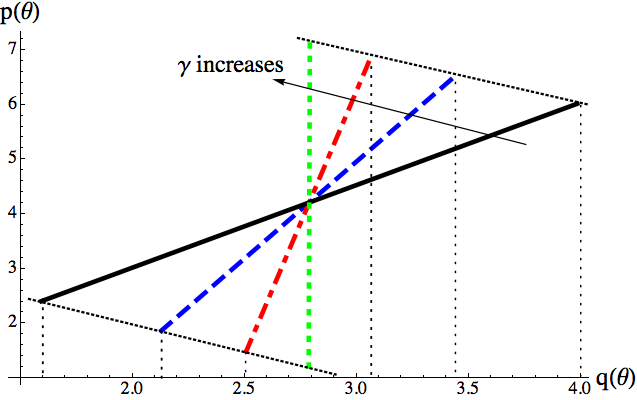
\includegraphics[width=10.cm]{figch1/monopoly_complet.png}\label{monopsup}}\quad
\subfigure[\small{$S^{-1~*}(p)$}]{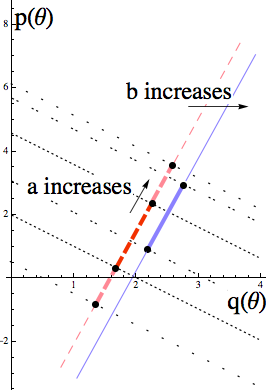
\includegraphics[width=4.5cm]{figch1/monopoly_completab.png} \label{monopab}}}
\captionsetup{singlelinecheck=off}
\caption[a b]{\small{ \textbf{\subref{monopsup}} Four optimal supply schedules are plotted. In black (full line) $\gamma=0$. As $\gamma$ increases we transition from the black curve to the blue curve (large dashes), then the red curve (mixed dashes) and then finally for $\gamma\to\infty$ to the green one (small dashes). The range of production is highlighted for each curve through the thin vertical dotted lines. 
\vspace{0.1cm}

\textbf{\subref{monopab}} The thin black dotted lines represent the extremal demand functions given $a$ and $b$, i.e. $D(\underline{\theta},p)$ and $D(\overline{\theta},p)$. From \ldots to \ldots $b$ is kept fixed while $a$ is increased, and from \ldots to \ldots $a$ is kept constant while $b$ is increased. In red (dashed) the solution for a given value of $b$. As $a$ increases, the solution widens from the thick deep red region to the thick light red one. In the case for which $a$ is kept constant and $b$ is increased the solution shifts from the dashed deep red region to the full thick blue one.   
}} 
\label{fig:monop}
\end{figure}

\section{The Symmetric Oligopoly}\label{oligosolve}

We keep the same linear demand specification as in the monopoly, therefore, with $n$ competitors one has to consider the residual demand faced by each producer: 
\begin{flalign}
&S(p(\theta))=a\theta+b-(n-1)S(p(\theta))-p&\label{condsymi}\\
&S(p(\theta))=\frac{a\theta+b-p}{n} &\label{supequ}\\
&S'(p(\theta))=\frac{a-\dot{p}}{n\dot{p}}&\\
&S''(p(\theta))=-\frac{a\ddot{p}}{n\dot{p}^3}&\label{condsymf}
\end{flalign} 
For concision, we drop the explicit dependencies of the different functions on their arguments in the following equations; $f(\theta)$, $p(\theta)$ and $S(p(\theta))$ will be noted $f$, $p$ and $S$ respectively. The maximisation program now writes:
\begin{equation}
%\begin{split}
\displaystyle{\max_{p(\cdot)}}~\int_{-1}^{1} f\bigg(p(a\theta+b-p-(n-1)S) -\frac{\lambda}{2}(a\theta+b-p-(n-1)S)^2%\\
-\frac{\gamma}{2}(1-\theta^2) \left(a-\dot{p}(1+(n-1)S')\right)^2\bigg)d\theta
%\end{split}
\label{maxoligopo}
\end{equation}
\begin{eqnarray}
s.t.\hspace{2cm}&\dot{p}\in[0,a] \nonumber\\
&p\leq a\theta+b \nonumber
\end{eqnarray}
with, as before, $\dot{X}=\frac{dX}{d\theta}$ and $X'$ is the derivative of function $X$ with respect to its argument. 

\subsection*{Results}
\begin{proposition}\label{propoligo1}
The solution exists, is unique, and has the following form:
\begin{equation}
\forall \theta \in [-1,1],~p^*(\theta) =aK_1\theta+bK_2 \label{oligosol}
\end{equation}
with 
\begin{flalign}
&\displaystyle{K_1=\frac{n\sqrt{(4\gamma+\lambda+n)^2-4n+4}-(4\gamma+\lambda+n)(n-2)}{2(4\gamma+\lambda+2n)}}& \\
&\displaystyle{K_2=\frac{\lambda(n-1)+K_1(\lambda+n)}{(\lambda+n)(n-1)+K_1(\lambda+2n)}}&
\end{flalign}
and the supply schedule has the following expression:
\begin{flalign}
&S^*(p)=\frac{1}{n}\left( p\left( \frac{1}{K_1}-1\right)+b\left( 1-\frac{K_2}{K_1}\right) \right)&
\end{flalign}
\end{proposition}
\begin{proof}
 See Annex \ref{annex1}. \qed
\end{proof}

We are now going to focus on the graphical representation of these solutions. As in the monopoly case we obtain unique solutions of increasing steepness in the ramping cost parameter $\gamma$. When the ramping costs increase, it becomes more and more costly to allow for a large domain of potential quantities to be produced. \\

The black curve in Fig.~\ref{fig:oligop} corresponds to the limit solution when $\gamma\to0$, for which the problem gets closer to that of KM, i.e. no ramping costs. Note that as long as $\gamma\neq0$ the solutions are unique, thus our framework does not converge to that of KM.\\

\begin{proposition}
When $\gamma\to0$, the solution remains unique and converges towards the linear schedule available in KM's set of solutions, that is the same schedule selected with KM's selection rule obtained when considering an infinite support for the shocks.
\end{proposition}
\begin{proof}
It is straightforward to check that $K_1$ and $K_2$ have the same values as KM for $\gamma\to0$. \\
More intuitively the argument is as follows. When $\gamma\to 0$, with $\gamma>0$, we retain a unique solution although the problem itself converges towards that of KM. We should select an equilibrium present in KM's continuum. When KM take the limiting case of an infinite support of shocks they select a unique equilibrium. In our case we can do the same thing by taking $a\to\infty$. In the limit, our solution being in their set which converges to a unique equilibrium, those two selected equilibria should be equal. Now note that our solution does not depend explicitly on $a$ so that when the support is finite, we still select the same equilibria out of what is now a continuum of equilibria in KM's framework.             \qed
\end{proof}


\begin{figure}[h] 
\centering
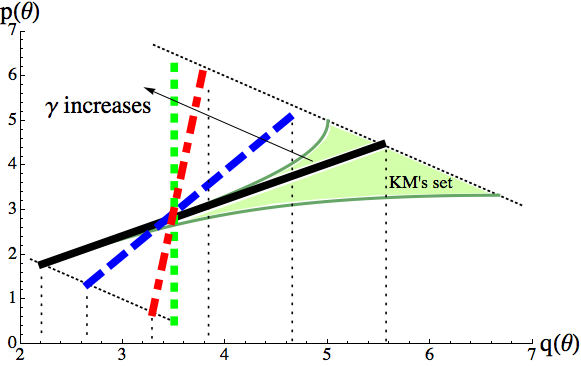
\includegraphics[width=12cm]{figch1/oligovraiKMd.png}
\caption{\small{This graph plots $S^*(p)$ for different values of the ramping cost parameter, and compares them to the set of equilibria obtained in KM's framework. Four optimal supply schedules are plotted. The black curve (full line) corresponds to the case where $\gamma\to0$. As before, as $\gamma$ increases the optimal schedules get steeper and steeper until in the limit of $\gamma\to\infty$, the optimal schedule attains a vertical slope. In addition, we show the set of available equilibria in KM's model in light green, and the extremal demand schedules in dashed black.  }} \label{fig:oligop}
\end{figure}

Intuitively, as we take $\gamma$ to $0$ we come closer to the situation captured in KM, but as long as $\gamma>0$, the producer still faces dynamic costs, and therefore converges towards the only linear schedule available in KM's set, as shown in Fig.~\ref{fig:oligop}, in which we plot our solutions on top of KM's solution set in order to clarify the comparison. \\

Note that it isn't possible to transition smoothly from our model to that of KM, although they are obviously closely related. Indeed, $\forall \gamma>0$, our model yields unique solutions, but for $\gamma=0$ we return to KM's model for which there is a continuum of equilibria. There is an intrinsic discontinuity between these two models, namely, the correspondence $\Gamma(\gamma)$ associating the set of equilibria to the symmetric oligopoly problem obtained for a given value of the ramping cost parameter $\gamma$ is not lower hemicontinuous at $\gamma=0$. \\

In addition to proposing a way to take into account dynamic technological constraints, our model provides a selection rule to choose from the continuum of equilibria described in KM's seminal work, i.e. the solutions' stability to ramping costs.\\

We have here a model which solutions depend on the distribution of shocks, therefore we are able to capture the interday variation of bids by assuming that the distribution of shocks varies from day to day. In this case, there exists only one symmetric equilibria each day, function of the distribution of shocks.\\

In the next section we are going to present how to capture richer dynamics, and especially how the surface of bids should evolve with time when the producers have information about the anticipated variation of shocks during the day. 



\section{Dynamic behavior of the bids} \label{dynamics}
On the day-ahead market, bids, although made once per day for each period included in the next 24 hours, vary from one another. This is because demand is expected to vary according to a daily cycle with, roughly speaking, low demand during the night and higher demand during the day. The model described above doesn't account for these hourly dynamics. Here we present a way to capture these intraday variations, by considering bids that depend continuously on the date $t$. \\

Previously, the SDE defining the dynamics of the problem was written as: 
$$d\theta(t)=-2\theta(t) dt+\sqrt{1-\theta(t)^2}dB_t$$ 
 This specification implies a stochastic trajectory for the shocks, bounded by a constant envelope. \\

To account for these intraday variations we define the envelope by two functions, $(\underline{\theta}(t),\overline{\theta}(t))$, respectively the lower and upper bounds of the shocks. These two functions, although very easy to comprehend, are not the most useful way to define the boundary. Instead we are going to use the average value of the shocks, and the half width of the envelope, $(\hat{\theta}(t), \omega(t))$. This means that $\underline{\theta}(t)=\hat{\theta}(t)-\omega(t)$ and $\overline{\theta}(t)=\hat{\theta}(t)+\omega(t)$. The only restriction we impose on the envelope is that we require it to be continuously differentiable, that is $(\hat{\theta}(t),\omega(t))\in\mathcal{C}^1(\mathbb{R})$.\\

Consider the following SDE, in which we drop the explicit dependency of the different functions on time, that is $\theta(t)$, $\hat{\theta}(t)$ and $\omega(t)$ will be noted $\theta$, $\hat{\theta}$ and $\omega$:
\begin{equation}
\begin{split}
  d\theta=\left[(\hat{\theta}-\omega-\theta)+\left(1+\frac{\tau}{\omega}\frac{d\omega}{dt_r}\right)(\hat{\theta}+\omega-\theta)+\tau\left(\frac{d\hat{\theta}}{dt_r}-\frac{d\omega}{dt_r}\right)\right]\cdot dt_r\\+\sqrt{\left(1+\frac{\tau}{\omega}\frac{d\omega}{dt_r}\right)(\theta-\hat{\theta}+\omega)(\hat{\theta}+\omega-\theta)}\cdot dB_{t_r}
\end{split}
\end{equation}
with $\tau$ a rescaling parameter allowing to change the rate at which the brownian process blurs information pertaining an initial condition. This parameter is of the order of the cutoff timescale $\Delta t_c$ (a few seconds at most). We rescale time as we change this parameter, so that time $t$ and the rescaled time $t_r$ verify $t=\tau t_r$. By assumption, $\Delta t_c$ is much smaller than the typical timescale of variation of strategies, therefore by hypothesis $\left(1+\frac{\tau}{\omega}\frac{d\omega}{dt_r}\right)>0$. The distribution of the shocks can be obtained through Fˆkker-Planck's equation \ref{FokP} and we obtain:
$$f(\theta,t_r)=\frac{6}{\omega(t_r)^3}(\theta(t_r)-\hat{\theta}(t_r)+\omega(t_r))(\hat{\theta}(t_r)+\omega(t_r)-\theta(t_r))$$

\subsection{Results}
\subsubsection{Monopoly dynamics}
\begin{proposition}\label{monopropdyn}
In the case of an envelope evolving with time, that is shocks belong to the bounded support $[\hat{\theta}-\omega,\hat{\theta}+\omega]$, there exists a unique optimal solution to the monopoly problem. It can be expressed as:
\begin{flalign}
&p^*=\frac{4\gamma\left(1+\frac{\tau}{\omega}\frac{d\omega}{dt}\right)+1+\lambda}{4\gamma\left(1+\frac{\tau}{\omega}\frac{d\omega}{dt}\right)+2+\lambda}\cdot\theta-\frac{4\gamma\left(1+\frac{\tau}{\omega}\frac{d\omega}{dt}\right)}{(2+\lambda)\left(4\gamma\left(1+\frac{\tau}{\omega}\frac{d\omega}{dt}\right)+1+\lambda\right)}\cdot\hat{\theta}&\label{monopdynp}
\end{flalign}
The corresponding optimal supply schedule writes as:
\begin{flalign}
&S^*(p)=\frac{1}{4\gamma\left(1+\frac{\tau}{\omega}\frac{d\omega}{dt}\right)+1+\lambda}\left(p+\frac{4\gamma\left(1+\frac{\tau}{\omega}\frac{d\omega}{dt}\right)}{2+\lambda}\cdot\hat{\theta}\right)&\label{monopdynS}
\end{flalign}
\end{proposition} 
\begin{proof}
See appendix \ref{monopdyn}, to be written. \qed
\end{proof}

We start by describing the dynamics of the monopoly case because the oligopoly case is not richer dynamically, but it is more complex to describe. Note that if $\frac{d\omega}{dt}=0$ equations \ref{monopdynp} and \ref{monopdynS} are equal to equations \ref{monopsol} and \ref{monopS} respectively as expected. \\
         
The optimal supply schedule depends on the relative rate of change of the width $\frac{1}{\omega}\frac{d\omega}{dt}$ and on the average shock $\hat{\theta}$. More precisely, with a constant width, the optimal supply schedule varies according to variations in the expected average value of the shocks. This is quite standard, if demand is higher, the price and quantities both increase, and here this increase occurs with a constant slope. The behavior of the supply schedule when the width varies is less trivial. \\

Remember that when describing the slope of the schedule, we are considering the plane $(quantity, price)$ while the schedule as defined by $S^*(p)$ represents the same curve but in the plane $(price, quantity)$. An increase in width is equivalent to a higher ramping cost parameter while a decrease in width is equivalent to a lower ramping cost parameter. These results are illustrated in Fig. \ref{figdyn1}. \\

To understand the economic intuition behind this result, consider first an increase in the width of the envelope at date $t_1$.  Consider now one possible value of $\theta(t_1)$. At $t_1+dt$, had the width been constant there would have been a given level of uncertainty about the values that $\theta(t_1+dt)$, and thus the ramping costs, could have taken.  If the width of the envelope is increasing then there is more uncertainty regarding the potential values that could be taken by $\theta(t_1+dt)$, therefore more expected ramping costs incurred, and a higher slope to hedge these costs. On the other hand, when the width decreases, the situation is reversed. In that case, we move towards a situation in which there is less uncertainty about the ramping costs, so that the slope is smaller than for a constant envelope. This difference between increasing and decreasing width is illustrated by comparing the two regions of the envelope displayed in (full) black line in Fig. \ref{figdyn1}. In addition, when contrasting the left and the right side of the figure one sees that the change in the informativeness of the envelope is captured by the relative change of the width: for the same rate of change, if the width is larger (right) then the change in informativeness is smaller (the change in the area captured by the (dashed) red and (full) green arrows).  \\

\begin{figure}[h] 
\centering
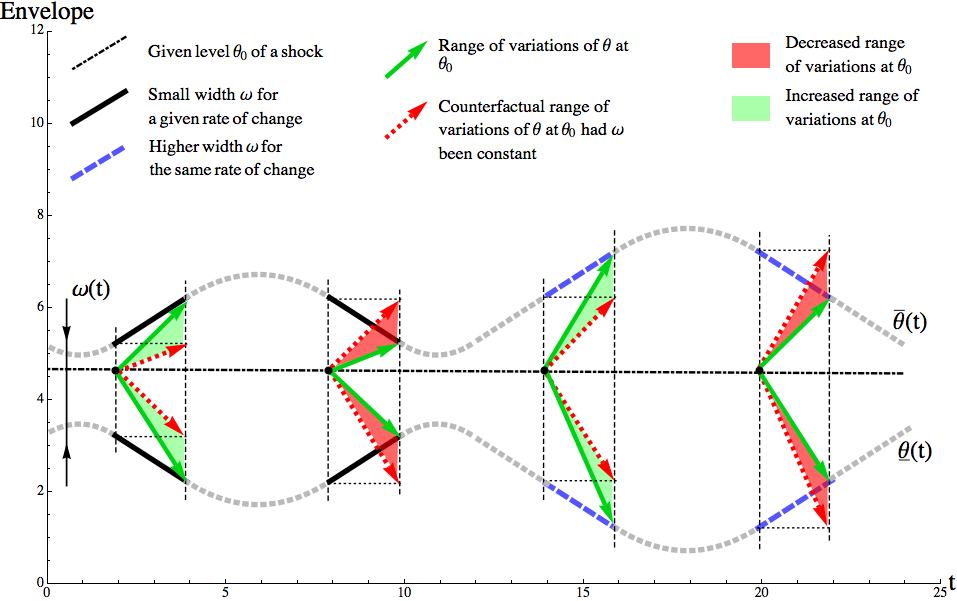
\includegraphics[width=15cm]{figch1/figdyn1.png}
\caption{\small{This graph plots an envelope of constant average value but varying width $\omega(t)$. By comparing regions of increasing or decreasing width, respectively the left or right side of a lobe, one sees that the informativeness of the envelope is being respectively reduced or increased with respect to a situation where the width would be kept constant. The change in informativeness is represented by the area between the (full) green arrows (observed level of informativeness) compared to the area between the (dashed) red arrows (level of informativeness had the width been constant). In addition, by comparing the left lobe to the right one, it is possible to see why the relative variation of the width, and not the absolute variation of the width, matters. For a larger width (right lobe) and the same rate of change in the width, there is less change in informativeness than for a smaller width (left lobe), i.e. the same rate of change matters less for the right lobe than for the left lobe. }} \label{figdyn1}
\end{figure}

\newpage
\subsubsection{Oligopoly dynamics}
\begin{proposition}\label{oligodynp}
The solution exists, is unique, and has the following form:
\begin{equation}
\forall \theta \in [-1,1],~p^*(\theta) =aK_1(t)\theta+bK_2(t) 
\end{equation}
with 
\begin{flalign}
&\displaystyle{K_1(t)=\frac{n\sqrt{\left(4\gamma\left(1+\frac{\tau}{\omega}\frac{d\omega}{dt}\right)+\lambda+n\right)^2-4n+4}-\left(4\gamma\left(1+\frac{\tau}{\omega}\frac{d\omega}{dt}\right)+\lambda+n\right)(n-2)}{2\left(4\gamma\left(1+\frac{\tau}{\omega}\frac{d\omega}{dt}\right)+\lambda+2n\right)}}& \\
&\displaystyle{K_2(t)=\frac{\lambda(n-1)+K_1(t)(\lambda+n)}{(\lambda+n)(n-1)+K_1(t)(\lambda+2n)}}&
\end{flalign}
and the supply schedule has the following expression:
\begin{flalign}
&S^*(p,t)=\frac{1}{n}\left( p\left( \frac{1}{K_1(t)}-1\right)+\hat{\theta}\left( 1-\frac{K_2(t)}{K_1(t)}\right) \right)&\label{dynsupply}
\end{flalign}
\end{proposition}
\begin{proof}
 See Annex \ref{oligodyn}, to be written. \qed 
\end{proof}

The dynamic behavior is the same as that of the monopoly situation presented above, and variations of the optimal schedule with respect to the other parameters are the same as in the case of a constant envelope, as described in section \ref{oligosolve}. 

%We now plot optimal schedules in the case where the width $\omega$ is kept constant and in the case where the average shock $\hat{\theta}$ is kept constant. \\
%
%INSERT FIGURE HERE

%\subsubsection{Generalisation of the distribution}
%Up until now we have considered a quadratic distribution of shocks. Our results can still be expressed in closed form when we allow the distribution to be free in the set of Generalised Beta distributions, that is, rougly speeking, polynomial distributions with only one lobe. This allows for asymetric distributions to be considered, although it is not the point of this article to describe the effects of the assymetry of the distribution of shocks on the shape of the optimal supply schedules. \\
%
%EXPRESSION GENERALISED BETA + PROOF
%
\section{Discussion}\label{disc}

DIFFERENTIATING DAY-AHEAD AND INTRADAY MARKETS.\\
TRANSITION BETWEEN KM AND THIS MODEL FOR DISCRETE TIME AND RAMPING COSTS: RATE OF CONVERGENCE TOWARDS THE UNIQUE SOLUTION OF THE CONTINUOUS CASE?

\section{Concluding Remarks}\label{ccl}

By introducing technological constraints previously neglected we are able to take into account the effects of the dynamics of demand shocks on the supply function framework. We restrict ourselves to linear demand. The optimal supply schedules obtained are unique, and their slope increase with the ramping costs, congruent with the idea that too much variation in production is costly. We also capture the dynamics of the bids themselves. \\

Although mathematically more demanding than the traditional model by Klemperer and Meyer, we consider that this new model, while conceptually sparing (we only add ramping costs) allows for a richer, more realistic description of the electricity market, and opens new research avenues.  It yields precise and testable predictions on the dynamics of the electricity market with tractable functional forms, at least in the linear demand case. In addition, by explicitly modeling the dynamics, our work opens the possibility to explore interactions between intraday and day-ahead markets, markets that were indistinguishible in the previous framework. We are also able to account for negative prices which was impossible in the previous framework. Such negative prices are actually observed, although rarely, on the market: producers prefer to subsidize consumption instead of decreasing it by a lot. \\

Next, we want to generalize the existence and uniqueness results to non linear demand functions and develop more comprehensive comparative statics. It would also be important to study the robustness of our solutions to modifications of the general form of the stochastic differential equation governing the dynamics of the system. Finally, and more generally, we think that this concept of dynamic costs, the fact that change is costly, is ubiquitous and could fuel interesting research into the dynamics of a large range of markets. Such avenues have been pursued in the case of stochastic optimal control, that is, instantaneous reactions to stochastic shocks. Here we are describing a market on which agents are forced to optimize in advance, so that they have to react to continuous changes in the anticipated shocks, but not the shocks themselves, which can be understood as stochastic optimisation with periodic commitment. 

%\bibliographystyle{te}
%\bibliography{biblio}

\begin{subappendices}
\section*{Appendix}
\addcontentsline{toc}{chapter}{Appendix}
\numberwithin{figure}{section}
\numberwithin{equation}{section}

\section{Proof of Proposition \ref{monopequilibria} \label{annexmonop}}
Define the following Hamiltonian: 
\begin{equation}
\begin{split}
H(p(\theta),\dot{p}(\theta),\mu(\theta),\theta)= f(\theta)\bigg( p(\theta)(a\theta+b-p(\theta))-\frac{\lambda}{2}(a\theta+b-p(\theta))^2\\
-\frac{\gamma}{2}(1-\theta^2)\left(a-u(\theta)\right)^2\bigg)+\mu(\theta) u(\theta)
\end{split}
\end{equation}
where $u(\theta)$ is the control variable defined through the following equation of motion: $u(\theta)=\dot{p}(\theta)$, $u(\theta)\in[0,a]$. We do not consider the non-negative demand constraint and will check ex-post that our solution verifies this condition. \\

Now note that:
\begin{eqnarray}
\forall\theta\in(-1,1),&\displaystyle{\frac{\partial^2 H}{\partial p^2}}=-(2+\lambda)f(\theta)<0\label{concmono1}\\
&\displaystyle{\frac{\partial^2 H}{\partial u^2}}=-\gamma(1-\theta^2)f(\theta)<0\label{concmono2}
\end{eqnarray}
The Hamiltonian is therefore strictly concave in $p(\theta)$ and $u(\theta)$. Let $(p^*(\theta),u^*(\theta))$ be an admissible pair to the problem, that is a pair such that $u^*(\theta)=\dot{p}^*(\theta)$. If there exists a continuous and piecewise continuously differentiable function $\mu(\theta)$ such that: 
\begin{flalign}
\dot{\mu}(\theta)=-\frac{\partial H}{\partial p}^*\hspace{1.65cm}\label{mupmonop}\\
\mu(-1)=\mu(1)=0 \hspace{1.13cm}& \textrm{in order for prices to be free at the boundaries}\label{monopbound}\\
\forall (\theta,u)\in[-1,1]\times[0,a],\hspace{0.17cm}& \frac{\partial H}{\partial u}^*(u^*(\theta)-u)\geq0\label{mangaham}
\end{flalign}
with $\frac{\partial H}{\partial u}^*=\frac{\partial H}{\partial u}(p^*(\theta),u^*(\theta),\mu(\theta),\theta)$, then the Mangasarian sufficiency theorem ensures that $(p^*(\theta),u^*(\theta))$ is the optimal solution \cite[p.105]{constraint}. Let us check that eq.~\ref{monopsol} defines the optimal solution.\\

Equation \ref{mupmonop} defines $\mu(\theta)$ up to a constant. Through direct integration we obtain: $$\mu(\theta)=3a\left( (2+\lambda)\frac{4\gamma+1+\lambda}{4\gamma+2+\lambda}-1-\lambda\right)(2\theta^2-\theta^4)+const.$$
This expression is symmetric in $\theta$ therefore by choosing the adequate value for the constant, we ensure that eq.~\ref{monopbound} is satisfied. The slope of the proposed $p^*$ is in $[0,a]$ therefore eq.~\ref{mangaham} requires $\frac{\partial H}{\partial u}$ to be null.  
\begin{eqnarray}
\forall \theta \in [-1,1],~ \frac{\partial H}{\partial u}=0\implies \frac{d}{d\theta}\frac{\partial H}{\partial u}=0\hspace{3.6cm}\nonumber\\
\textrm{i.e. }\displaystyle{\dot{u} (\theta)= -\frac{4\theta}{1-\theta^2}(a-u(\theta))-\frac{(1+\lambda)(a\theta+b)}{\gamma(1-\theta^2)}+\frac{(2+\lambda)p (\theta)}{\gamma(1-\theta^2)}}
\end{eqnarray}
It is straightforward to see that the proposed solution satisfies this differential equation, thus we know that $\frac{\partial H}{\partial u}$ is a constant and as $\mu(-1)=0$ it is in fact null. Lastly,  we see that $p^*(\theta)\leq a\theta +b$.\\

The proposed $p^*(\theta)$ therefore defines the unique optimal supply function, i.e. the parametrized curve $(a \theta +b-p^*(\theta),p^*(\theta))$.

\section{Proof of Proposition \ref{propoligo1} \label{annex1}}
As for eq.~\ref{maxoligopo}, for the sake of concision, we do not write the explicit depencies of the different functions on $\theta$, thus $f(\theta)$, $p(\theta)$, $u(\theta)$, $\mu(\theta)$ and $S(p(\theta))$ will be written as $f$, $p$, $u$, $\mu$ and $S$ respectively. Define the following Hamiltonian: 
\begin{equation}
\begin{split}
H(p,u,\mu,\theta)= f\bigg( p(a\theta+b-p-(n-1)S)-\frac{\lambda}{2}(a\theta+b-p-(n-1)S)^2\\
-\frac{\gamma}{2}(1-\theta^2)\left(a-u(1+(n-1)S')\right)^2\bigg)+\mu u
\end{split}
\end{equation}
where $u$ is the control variable defined through the following equation of motion: $u=\dot{p}$, $u\in[0,a]$. We do not consider the non-negative demand constraint and will check ex-post that our solution verifies this condition. \\

If a symmetric equilibria exists, eqs.~\ref{condsymi} through~\ref{condsymf} imply that the regular conditions for an admissible pair to be optimal write  :
\begin{flalign}
&u=\dot{p}\in[0,a]&\\
&\partial_uH<0\implies u=0&\\
&\partial_uH>0\implies u=a&\\
\begin{split}\partial_uH=0\implies u\in[0,a]\textrm{ and} \hspace{6cm}\\
\ddot{p}=-\frac{4\theta(a-\dot{p})}{1-\theta^2}-\frac{\lambda(a\theta+b-p)}{\gamma(1-\theta^2)}-n\frac{\dot{p}(a\theta+b-2p)-a(n-1)p}{\gamma(1-\theta^2)(a(n-1)+\dot{p})}
\end{split}\label{oligoequadiff}\\
&\dot{\mu}=-\partial_pH&\\
&\mu(-1)=\mu(1)=0&\label{oligobc}
\end{flalign}
It is easy to check that $(K_1,K_2)\in(0,1)$ and that the solution~\ref{oligosol} solves eq.~\ref{oligoequadiff} subject to the boundary conditions~\ref{oligobc}. The supply schedule is therefore also linear, with equation :
\begin{flalign}
& S(p)=\frac{1}{n}\left( p\left( \frac{1}{K_1}-1\right)+b\left( 1-\frac{K_2}{K_1}\right) \right)&\label{oligoS}
\end{flalign}
We can now use the Mangasarian theorem to obtain that our admissible pair is indeed solution, $H(p,u,\mu,\theta)$ being concave in $(p,u)$ for linear supply schedules. However the Mangasarian cannot yield that this solution is unique because for a symmetric equilibria, if supply schedules are modified, the hamiltonian changes alongside and we are faced with a new maximisation program. \\

To obtain that the solution is unique we are going to show explicitly that no other candidate solution exists. \\

First, note that :
\begin{flalign}
\begin{split}
\dot{\mu}=-f\bigg( \frac{a\theta+b-2p}{n}-a\frac{(n-1)p}{n\dot{p}}\hspace{5cm}\\
+\lambda\frac{a\theta+b-p}{n}\cdot\frac{a(n-1)+\dot{p}}{n\dot{p}}-\gamma(1-\theta^2)(n-1)\frac{a-\dot{p}}{n}\cdot\frac{a\ddot{p}}{n\dot{p}^2}\bigg)\label{oligomup}
\end{split}
\end{flalign}
If $(p^*,u^*)$ maximises the program then the maximum principle implies that there exists a continuous and piecewise continuously differentiable function $\mu$, as shown in \cite[Theorem 2 p.85]{constraint}. This combined with the above equation implies that $\dot{p}\neq0$ a.e.\\

Assume now a solution of the form $\forall\theta\in[-1,1],~p=a\theta+\beta$, by injecting this expression in eq.~\ref{oligomup} there is no $\beta$ such that  the boundary conditions~\ref{oligobc} are verified. \\

In addition:
\begin{flalign}
&\forall\theta\in(-1,1),~\displaystyle{\frac{\partial^2 H}{\partial u^2}}=-f\gamma(1-\theta^2)(1+(n-1)S')^2<0\label{concoligo}&
\end{flalign}
The Hamiltonian is therefore strictly concave in $u$ and $[0,a]$ is convex. These two properties yield that $u^*$ is continuous, as shown in \cite[Note 2.b. p.86]{constraint}. We have proved the following result :
\begin{lemma}
For any symmetric equilibrium $\exists A\subseteq[-1,1]$ s.t. A is the union of segments of $[-1,1]$ and $\forall\theta\in A$, $\partial_u H=0$ 
\end{lemma}

Assume the following hypothesis is true, $H_1:\exists\theta_c\in(-1,1)$ s.t. $[-1,\theta_c]\subseteq A$, then knowing that $\dot{p}\in\mathcal{C}^0([-1,1],[0,a])$ we can rewrite differential equation \ref{oligoequadiff} around the value $\theta=-1$ by defining $\theta=-1+\epsilon$ with $\epsilon=o(1)$:
\begin{flalign}
&\frac{d^2p}{d\epsilon^2}= \frac{C}{\epsilon}+o(1) \textrm{ with }C\neq0 \textrm{ if }p(\theta)\neq aK_1\theta+bK_2&
\end{flalign}
This means that locally around $-1$, any solution to eq. \ref{oligoequadiff} but solution \ref{oligosol} diverges. Hypothesis $H_1$ is therefore wrong and $\exists\theta_c\in(-1,1)$ s.t. $\forall\theta\in[-1,\theta_c]$, $\exists \beta$ s.t. $p(\theta)=a\theta+\beta$.\\

At $\theta_c$ we have $\partial_u H=0$ and as $\dot{p}$ is continuous, $\dot{p}(\theta_c)=a$. For the solution to be interior we need $\ddot{p}(\theta_c)\leq0$. 
\begin{flalign}
&\partial_{\dot{p}}H(p,\dot{p},\mu,\theta_c)=0\Leftrightarrow \mu(\theta_c)=0&\\
&\ddot{p}(\theta_c)\leq0\Leftrightarrow b(1+\lambda)-\beta(n+1+\lambda)\geq na\theta&
\end{flalign}
Straightforward computations show that both conditions are mutually exclusive, therefore there doesn't exist another candidate symmetric equilibria, and our solution is unique.\\

Lastly, to compute the optimal supply function, we inverse the optimal price in order to get the shock as a function of the price at the equilibrium, and we inject this expression in Eq. \ref{supequ}.

\section{Proof of proposition \ref{monopropdyn}}\label{monopdyn}

\section{Proof of proposition \ref{oligodynp}}\label{oligodyn}
%\section{Stochastic process} \label{rampingcostsappendix}
%
%\subsection{The ramping costs}
%In the rest of the paper we are going to consider quadratic ramping costs. More precisely we consider the costs induced by fluctuations in the production level. As described in the introduction, fluctuations imply increased wear and tear, whether the production is increasing or decreasing. In addition, these ramping costs are null in the absence of fluctuations. This means that they can be captured by a function $C_r(\cdot)$ verifying $C_r(0)=0$, $C_r(\cdot)\geq0$ and increasing in the absolute value of its argument. In the abscence of more detailed knowledge about the actual shape of these ramping costs, it seems reasonable to consider a quadratic cost function, that is the first term in a Taylor expansion of the actual real ramping cost function. \\
%
%We cannot compute $\frac{d\theta}{dt}$ as it appears in Eq.~\ref{maxbase}, as a stochastic process, although everywhere continuous, is nowhere differentiable. We are therefore going to consider a random walk of timestep $\Delta t$ which converges towards the It\={o} process \ref{sdegen}, using the Euler-Maruyama approximation, a generalisation of the Euler method to stochastic differential equations. We consider a Markov chain $Y$ defined as follows : 
%
%\begin{equation}
%\Delta Y_n=Y_{n+1}-Y_n= \mu(Y_n,n \Delta t)\Delta t+\sigma (Y_n,n \Delta t)\Delta B_n
%\end{equation}
%where $\Delta B_n=B_{(n+1)\Delta t}-B_{n\Delta t}$. These $\Delta B_n$ are \emph{i.i.d.} normal random variables of mean $0$ and variance $\Delta t$. Note that as $\Delta t$ is taken towards $0$, this Markov chain converges towards its underlying stochastic process defined by eq.(\ref{sdegen}).\\
%
%The ramping costs are taken as quadratic in the variation of the production, so we compute the following quantity : 
%
%\begin{equation}
%\mathbb{E}\left[\left(\frac{Y_{n+1}-Y_n}{\Delta t}\right)^2\middle \vert Y_n  \right]=\frac{\sigma (Y_n,n \Delta t)^2}{\Delta t}
%\label{markovariation}
%\end{equation}
%
%which obviously diverges when the Markov chain is taken towards its underlying stochastic process. To overcome this issue we have to consider a technological constraint : below a given timescale, power plants do not face ramping costs anymore. Two distinct mechanisms justify this statement, both induced by the very nature of the ramping costs : wear and tear is due to the fluctuations of temperature in the core of the power plant. \\
%
%The first mechanism through which ramping costs disappear below a given timescale is that for fluctuations occurring on the typical timescale of the millisecond and below, the production does not actually fluctuate. If the consumption varies very rapidly, the frequency of the electric network automatically adjust, thus it is not even asked of the production to change. \\
%
%The second mechanism through which ramping costs vanish below a given timescale is that for fluctuations occurring on the typical timescale of the second and below, although the production does fluctuate, the temperature in the core of the power plant does not. This comes form the thermal inertia of the materials forming the power plant. Fluctuations of consumption on these typical timescales, if they do imply a change in production, do not change the temperature in the core, and consequently do not imply ramping costs. This can be understood by using an everyday life analogy : lighting a stove is extremely quick, but the water being heated will take time to boil, because of its thermal inertia. \\
%
%Those two mechanisms effectively act as low-pass filters between the consumption on the network and the temperature in the core of the power plant, which bounds from below the timestep of the Markov process. In both cases, the typical timescales below which fluctuations become irrelevant (milliseconds or seconds), which we call the cutoff timescale $\Delta t_c$, are much smaller than the typical timescales of the change in strategies that we are trying to explain (hour). \\
%
%The ramping costs are written as a function of the production for convenience, although the fact that they actually depend on the temperature of the core is used to explain the existence of a cutoff timescale. We consider a Markov chain converging towards a stochastic process. From eq.(\ref{markovariation}) we see that this approach leads to diverging ramping costs, and that the cutoff timescale allows for a technologically driven argument for which these costs are actually finite.  \\
%
%Consider a transformation $T(\cdot)$ that we apply to the Markov chain $Y$. Then:
%\begin{equation}
%\mathbb{E}\left[\left(\frac{T(Y_{n+1})-T(Y_n)}{\Delta t}\right)^2\middle \vert Y_n  \right]= \mathbb{E}\left[\left(\frac{T(Y_{n+1})-T(Y_n)}{Y_{n+1}-Y_n}\cdot\frac{Y_{n+1}-Y_n}{\Delta t}\right)^2\middle \vert Y_n  \right]    
%\label{markovcomposed}
%\end{equation}
%
%And in the limit:
%\begin{equation}
%\lim_{\Delta t \to 0}\mathbb{E}\left[\left(\frac{T(Y_{n+1})-T(Y_n)}{\Delta t}\right)^2\middle \vert Y_n  \right]= T'(Y_n)^2 \lim_{\Delta t \to 0}\mathbb{E}\left[\left(\frac{Y_{n+1}-Y_n}{\Delta t}\right)^2\middle \vert Y_n  \right]    
%\label{limitmarkovcomposed}
%\end{equation}
%But here, the right hand side diverges. We consider that $\Delta t_c$ is sufficiently small to justify the final approximation we are going to make in order to describe properly the problem at hand. We assume that the ramping cost function, considering a generic shock process $\theta(t)$ of the type given in eq.(\ref{sdegen}), can be written as: 
%\begin{equation}
%\mathbb{E}\left[\left(\frac{\Delta S_i(p(\theta(t)))}{\Delta t_c}\right)^2\middle \vert \theta(t)  \right] = \mathbb{E}\left[\left(\frac{\Delta S_i(p(\theta(t)))}{\Delta \theta(t)} \frac{\Delta \theta(t)}{\Delta t_c}\right)^2\middle \vert \theta(t)  \right]  \approx S_i'(p(\theta(t)))^2\dot{p}(\theta(t))^2 \frac{\sigma(\theta)^2}{\Delta t_c}
%\label{markovtosde}
%\end{equation}
%with $X'$ the derivative of quantity X with respect to its argument, $\dot{X}$ its derivative with respect to $\theta$ and $\Delta X(t)=X(t+\Delta t_c)-X(t)$. This is equivalent to saying that $\Delta t_c$ is sufficiently small to approximate these increase rate of the supply and price functions by their derivatives, i.e. do a first order taylor expansion. Note that we considered here that the variance term $\sigma$ depends only on $\theta$ and not explicitly on $t$, which in turn implies that the strategy $S_i$ does not depend explicitly on $t$ either. \\
%
%Let us consider the case where the strategy and the variance depend explicitly on the time, and are thus written $S_i(p(\theta(t)),t)$ and $\sigma(\theta,t)$ respectively.  By using a first order expansion as before, the ramping cost function can be approximated as follows:
%\begin{eqnarray}
%\mathbb{E}\left[\left(\frac{\Delta S_i(p(\theta(t)),t)}{\Delta t_c}\right)^2\middle \vert \theta(t)  \right] &\approx& \partial_1S_i(p(\theta(t)),t)^2\dot{p}(\theta(t))^2 \frac{\sigma(\theta,t)^2}{\Delta t_c} +\partial_2 S_i(p(\theta(t)),t)^2\nonumber\\
%&&+2\partial_1S_i(p(\theta(t)),t)\partial_2 S_i(p(\theta(t)),t) \dot{p}(t)\mathbb{E}\left[\frac{\Delta \theta(t)}{\Delta t_c}\middle \vert \theta(t)  \right]
%\label{markovtimedep}
%\end{eqnarray}
%with $\partial_iX$ the partial derivative of quantity $X$ with respect to its $i^{th}$ argument. We are now going to develop an argument that we made earlier: $\Delta t_c $ is considered much smaller (millisecond to seconds) than the typical timescale of change in strategies we are trying to capture (hour). This directly justifies the fact that we are going to neglect the second and third terms in the right hand side of eq.(\ref{markovtimedep}). We consider that:
%\begin{equation}
%\mathbb{E}\left[\left(\frac{\Delta S_i(p(\theta(t)),t)}{\Delta t_c}\right)^2\middle \vert \theta(t)  \right]  \approx \partial_1S_i(p(\theta(t)),t)^2\dot{p}(\theta(t))^2 \frac{\sigma(\theta,t)^2}{\Delta t_c}
%\label{finalapprox}
%\end{equation}
%
%Now, we can write down the instantaneous expected value of the profit of producer $i$ if the demand shock is $\theta(t)$, $\pi^e_i(t)$, that is the profit that one expects to obtain when demand is at $\theta(t)$ given the expected value of the ramping costs:
%
%\begin{equation}
%\pi^e_i(t)= p(\theta(t))S_i(p(\theta(t)),t) - C_s(S_i(p(\theta(t)),t)) -\frac{\gamma_0}{2} \partial_1S_i(p(\theta(t)),t)^2\dot{p}(\theta(t))^2 \frac{\sigma(\theta,t)^2}{\Delta t_c}
%\label{instantprofit}
%\end{equation}
%
%Lastly we have to write down the expected profit for a day's worth of submitted strategies. Let us consider that the chosen unit of time is the day. Therefore, the total expected profit $\Pi^e_i$ writes: 
%
%\begin{eqnarray}
%\Pi^e_i&=&\int_0^1\mathbb{E}[\pi^e_i(t)]dt\nonumber\\
%&=&\int_0^1\int_{\underline{\theta}}^{\overline{\theta}}f(\theta,t)\left[p(\theta)S_i(p(\theta),t) - C_s(S_i(p(\theta),t)) -\frac{\gamma}{2} \partial_1S_i(p(\theta),t)^2\dot{p}(\theta)^2 \sigma(\theta,t)^2\right]d\theta dt
%\label{totprofit}
%\end{eqnarray}
%with $\gamma=\gamma_0/\Delta t_c$
%
%\subsection{Discussion of the approximations}
%We want a tractable mathematical formulation of the dynamic problem faced by producers on the electricity market. To achieve this we seek to describe the discrete real life problem by an approximated continuous one. We first use two technological facts: fluctuations in production are costly, but only up to a certain cutoff timescale.  We note that this cutoff timescale is much smaller than the typical timescale of the dynamics we try to capture. We then use two types of mathematical approximations. The first one is that we rely heavily on first order expansions of the different terms we have to compute. The second one stems from the existence of these two different timescales that allow us to neglect certain terms but not others in these first order expansions. From the very beginning of this work, we build a framework aimed at capturing the dynamics of the market and exploit some technological constraints in order to make simplifications. The consequence of this modelling strategy is that this model, by construction, will not be able to adress very short term economic questions. 
%
%\subsection{The maximisation program}
%Here, we consider that the dynamics of demand shocks are given by eq.(\ref{eqSDE}), and that therefore  $\sigma(\theta,t)^2=\sigma(\theta)^2=(1-\theta^2)$.\\
%
%We now introduce the different conditions that have to be satisfied by the various terms in this problem. First, on most electricity markets, schedules must be increasing, therefore here we take $S_i'(\cdot)\geq0$. Second, the aggregate demand is non negative as consumers do not have production facilities at their disposal: $D(\theta(t),p(\theta(t)))=\sum_iS_i(p(\theta(t)))\geq0$. Last, we consider that the shocks $\theta$ are ordered so that the demand is increasing in $\theta$, i.e. $\frac{\partial D}{\partial\theta}\geq0$, and that the price has to weakly increase with the shocks, i.e. $\dot{p}\geq0$. Our initial stochastic maximisation program can thus be rewritten as a regular optimal control problem: 
%
%\begin{equation}
%\displaystyle{\max_{S_i(p)}}~\int_{-1}^{1} f(\theta)\left(p(\theta)S_i(p(\theta)) -C_s(S_i(p(\theta)))-\frac{\gamma}{2}(1-\theta^2)\left(S_i'(p(\theta))\dot{p}(\theta)\right)^2\right)d\theta
%\end{equation}
%\begin{eqnarray} 
%s.t.\hspace{2cm}&S_i'(\cdot)\geq0 \nonumber\\
%&\dot{p}\geq0\\
%&D(\cdot,\cdot)\geq0 \nonumber\\
%\end{eqnarray}
%
%The next section solves this problem for a monopoly. 

%\subsection{Link between residuals and width}\label{reswidth}
%
%Here I compute the range of production that can be realised at a given time $t$.
%
%Extremal demand functions : $D_{extr}(p)=b\pm a-p$. At the equilibrium, the supply function obtained in Eq. \ref{dynsupply} must be equal to the demand. Therefore the extremal equilibrium points are obtained from the following equation :
%
%\begin{eqnarray}
%\frac{1}{n}\left( p^*_{extr}\left( \frac{1}{K_1(t)}-1\right)+\hat{\theta}\left( 1-\frac{K_2(t)}{K_1(t)}\right) \right)=b\pm a-p^*_{extr}\\
%p^*_{extr}=\frac{nK_1(t)(b\pm a)+\hat{\theta}(K_2(t)-K_1(t))}{1+(n-1)K_1(t)}
%\end{eqnarray}
%Therefore we can compute the extremal production values:
%\begin{eqnarray}
%\frac{1}{n}\left( p^*_{extr}\left( \frac{1}{K_1(t)}-1\right)+\hat{\theta}\left( 1-\frac{K_2(t)}{K_1(t)}\right) \right) =\frac{K_1(t)}{1+(n-1)K_1(t)}\left( b\pm a +\hat{\theta}\left( 1-\frac{K_2(t)}{K_1(t)}\right)\right)
%\end{eqnarray} 
%Define $\Delta Q(t)$ as the range of possible quantities produced. Then
%\begin{equation}
%\Delta Q(t)=\frac{2aK_1(t)}{1+(n-1)K_1(t)}
%\end{equation}
%Now we can ask how does this range, which is correlated with the absolute value of the error termes between predicted production and realised production, changes in time.
%\begin{eqnarray}
%\frac{d \Delta Q(t)}{dt}=\frac{\frac{d K_1(t)}{dt}}{(1+(n-1)K_1(t))^2}
%\end{eqnarray} 
%This quantity is of the sign of $\frac{d K_1(t)}{dt}$. For concision, note $\frac{1}{\omega}\frac{d\omega}{dt}=\frac{\omega'}{\omega}$ with $X'=\frac{dX}{dt}$
%\begin{equation}
%\frac{d K_1(t)}{dt}=\frac{2 \gamma  n \left(\frac{\omega'}{\omega}\right)' \left(n^2-4+n (4 \gamma(1+\frac{\omega'}{\omega}) +\lambda+4)-(n-2) \sqrt{(4 \gamma  (1+\frac{\omega'}{\omega})+\lambda +n)^2-4 n+4}\right)}{(4 \gamma(1+  \frac{\omega'}{\omega}) +\lambda +2 n)^2 \sqrt{(4 \gamma  (1+\frac{\omega'}{\omega})+\lambda +n)^2-4 n+4}}
%\end{equation}
%Thus, $sign\left(\frac{d \Delta Q(t)}{dt}\right)=sign\left(\frac{\omega'}{\omega}\right)'$
%$$\Delta Q=\frac{\omega K_1}{1+(n-1)K_1}$$\tiny
%$$\frac{d\Delta Q}{dt}=\frac{\omega'(t) \left(n \sqrt{\left(4 \gamma +\lambda +n+\frac{4 \gamma  \omega'(t)}{\omega(t)}\right)^2-4 n+4}+(2-n) \left(4 \gamma +\lambda +n+\frac{4 \gamma  \omega'(t)}{\omega(t)}\right)\right) \left(4 \gamma +\lambda +2 n+\frac{4 \gamma  \omega'(t)}{\omega(t)}\right)+\frac{4 \gamma  \left(\omega(t) y''(t)-\omega'(t)^2\right) \left(\frac{n \left(4 \gamma +\lambda +n+\frac{4 \gamma  \omega'(t)}{\omega(t)}\right)}{\sqrt{\left(4 \gamma +\lambda +n+\frac{4 \gamma  \omega'(t)}{\omega(t)}\right)^2-4 n+4}}-n+2\right) \left(4 \gamma +\lambda +2 n+\frac{4 \gamma  \omega'(t)}{\omega(t)}\right)}{\omega(t)}-\frac{4 \gamma  \left(\omega(t) y''(t)-\omega'(t)^2\right) \left(n \sqrt{\left(4 \gamma +\lambda +n+\frac{4 \gamma  \omega'(t)}{\omega(t)}\right)^2-4 n+4}+(2-n) \left(4 \gamma +\lambda +n+\frac{4 \gamma  \omega'(t)}{\omega(t)}\right)\right)}{\omega(t)}}{2 \left(4 \gamma +\lambda +2 n+\frac{4 \gamma  \omega'(t)}{\omega(t)}\right)^2}$$












%\newpage
%\subsection{Symmetric oligopoly with general demand and cost functions}
%Assume that the inertial cost function has the property that $C_i(A\cdot B)=C_i(A)\cdot C_i(B)$, that is $C_i$ is a power function, or, more generally, consider any analytical function on $\mathbb{R}$, and as before, $\dot{X}=\frac{dX}{d\theta}$. Given a price $p(t)$ at date $t$, the instantaneous profit can be written as : 
%\begin{equation}
%\begin{split}
%\Pi(t)=p(t)\big[D(\theta(t),p(t)) -(n-1)S(p(t)) \big]-C_s\big(D(\theta(t),p(t)) -(n-1)S(p(t)) \big)\\
%-C_i\big(\dot{D}(\theta(t),p(t)) -(n-1)S'(p(t))\dot{p}(t) \big)C_i\bigg( \frac{d\theta}{dt}\bigg)
%\end{split}
%\end{equation}
%
%Demand is decreasing with price and we can always redefine and reorder the shocks so that demand is increasing with shocks: $\partial_p D\leq0$ and  $\partial_\theta D\geq0$. Along the equilibrium, we consider that the total production is weakly increasing in the shocks: $\dot{D}\geq0$. Lastly the price itself is weakly increasing in the shocks, so that $\dot{p}\geq0$. These two conditions can be summarized as $\dot{p}\in[0,-\frac{\partial_\theta D}{\partial_p D}]$ and lastly total production is always positive: $D\geq0$. Define $C_I(\theta,t)=\mathbb{E}\bigg[ C_i\bigg(\displaystyle{\frac{d\theta}{dt}}\bigg)\bigg|\theta,t \bigg]$. \\
%
%Let us start from the situation where the first $n-1$ producers bid the same supply function $S$. The maximization program of the $n^{th}$ producer writes:
%\begin{equation}
%\begin{split}
%\max_{p(\theta,t)}\int_{-1}^1 f(\theta,t)\bigg[ p\big[D(\theta,p) -(n-1)S(p) \big]
%-C_s\big(D(\theta,p) -(n-1)S(p) \big)\\
%-C_i\big(\dot{D}(\theta,p) -(n-1)S'(p)\dot{p} \big)C_I( \theta,t)\bigg]d\theta
%\end{split}
%\end{equation}
%s.t.
%\begin{flalign}
%&\dot{p}\in\left[0,-\frac{\partial_\theta D}{\partial_p D}\right]&\\
%&D\geq0&
%\end{flalign}
%
%
%
%
%
%\newpage
%At the symmetric equilibria we know that:
%\begin{flalign}
%&nS(p)=D(\theta,p) &\\
%&S'(p)=\frac{\dot{D}}{n\dot{p}}=\frac{\partial_\theta D+\partial_p D\dot{p}}{n\dot{p}}&\\
%&S''(p)=\frac{\ddot{D}\dot{p}-\dot{D}\ddot{p}}{n\dot{p}^2}=\frac{\dot{p}\partial_{\theta\theta}D+2\dot{p}^2\partial_{p\theta}D+\dot{p}^3\partial_{pp}D -\ddot{p}\partial_\theta D}{n\dot{p}^3}&
%\end{flalign}
%
%From optimal control theory we obtain that the maximizing $p(\theta)$ is solution of the following differential equation:
%\begin{equation}
%\begin{split}
%\ddot{p}=-\frac{n}{\partial_p D}\frac{C_i'\left( \frac{\dot{D}}{n}\right)}{C_i''\left(\frac{\dot{D}}{n} \right)} \left[ \frac{\dot{f}(\theta,t)}{f(\theta,t)}+\frac{C_I'(\theta,t)}{C_I(\theta,t)}\right]-\frac{\ddot{D}}{\partial_pD}-\frac{n\left(p-C_s\left( \frac{D}{n}\right)\right)}{\partial_pD~ C_I(\theta,t)C_i''\left( \frac{\dot{D}}{n}\right)}\\
%-\frac{nD\dot{p}}{\partial_pD(\dot{p}\partial_pD-(n-1)\partial_\theta D)C_I(\theta,t)C_i''\left( \frac{\dot{D}}{n}\right)}
%\end{split}
%\end{equation}
%
%\subsubsection{Unicity}
%The same exact reasonning as in the linear case shows that the solution is completely interior. 
%For $\theta=-1$ or $\theta=1$, we obtain the following boundary conditions: 
%\begin{equation}
%\begin{split}
%0=-nC_i'\left( \frac{\dot{D}}{n}\right)\left[ \frac{\dot{f}(\theta,t)}{f(\theta,t)}+\frac{C_I'(\theta,t)}{C_I(\theta,t)}\right](\dot{p}\partial_pD-(n-1)\partial_\theta D)C_I(\theta,t)\\
%-n\left(p-C_s\left( \frac{D}{n}\right)\right)(\dot{p}\partial_pD-(n-1)\partial_\theta D)-nD\dot{p}
%\end{split}
%\end{equation}
%Unless these two conditions are "colinear" (ex. $y''=-y$ with $y(0)=0=y(2\pi)$) the solution is unique. 
%
%\subsubsection{Existence}
%\begin{equation}
%\begin{split}
%\max_{p(\cdot)}\int_{-1}^1f[p(D-(n-1)S)-C_s(D-(n-1)S)-C_i(\dot{D}-(n-1)S'\dot{p})C_I]d\theta
%\end{split}
%\end{equation}
%
%Filipov yields that there always exists a best response. If we consider the application that for any supply curve $S$ on which the $n-1$ competitors agree on outputs the BR, then we can use a fixed point argument to obtain the existence of a symmetric equilibria.












%\begin{theorem}

%\end{theorem}
%\subsection{Oligopoly solution}
%\begin{itemize}
%\item Consider that the solution is of slope $a$ everywhere and is expressed as $p(\theta)=a\theta+\beta$. Then 
%\begin{flalign}
%\begin{split}
%\dot{\mu}=-f\bigg( \frac{a\theta+b-2p}{n}-\frac{a(n-1)p}{n\dot{p}} +\lambda(a\theta+b-p)\frac{a(n-1)+\dot{p}}{n^2\dot{p}}\\
%-\gamma\frac{1-\theta^2}{n\dot{p}^2}(a-\dot{p})(n-1)a\ddot{p}\bigg)\\
%\end{split}
%\end{flalign}
%\begin{flalign}
%\dot{\mu}=\frac{3a}{4}(\theta-\theta^3)-\frac{3(1+\lambda)}{4n}(b-\beta)(1-\theta^2)
%\end{flalign}
%so that 
%\begin{flalign}
%\mu=\frac{3a}{16}(2\theta^2-\theta^4)-\frac{3(1+\lambda)}{12n}(b-\beta)(3\theta-\theta^3)+const
%\end{flalign}
%We see that $\mu$ has odd terms in $\theta$, thus $\mu(-1)\neq\mu(1)$ unless $b=\beta$, in which case  it is a solution, with $0$ profit. 
%\item We check that \emph{ad hoc} functions of the form presented in Fig.~\ref{fig:oligop}, yield positive profits, thus $p(\theta)=a\theta+b$ is not the solution.
%\item $\mu(\theta)$ is absolutely continuous thus 
%\end{itemize}
%\subsection{Assymetric duopoly}
%Assume that $S_2(p)$ is linear, i.e. $S_2(p)=\alpha_2p+\beta_2$, and $S_1(p)+S_2(p)=a\theta+b-p$.
%\begin{equation}
%\begin{split}
%\max_{p}\int_{-1}^1f\bigg( p(a\theta+b-(1+\alpha_2)p-\beta_2)-\frac{\lambda}{2}(a\theta+b-(1+\alpha_2)p-\beta_2)^2\\
%-\frac{\gamma}{2}(1-\theta^2)(a-(1+\alpha_2)\dot{p})^2\bigg)\label{duopo}
%\end{split}
%\end{equation}
%s.t. $\dot{p}\in[0,\frac{a}{1+\alpha_2}]$ and $p\leq \frac{a\theta+b-\beta_2}{1+\alpha_2}$.\\
%
%Define:
%\begin{flalign}
%&p_0=\sqrt{1+\alpha_2}p&\\
%&a_0=\frac{a}{1+\alpha_2}&\\
%&b_0=\frac{b-\beta_2}{1+\alpha_2}&\\
%&\lambda_0=\lambda(1+\alpha_2)&\\
%&\gamma_0=\gamma(1+\alpha_2)&
%\end{flalign}
%Then the maximisation program~\ref{duopo} rewrites: 
%\begin{equation}
%\begin{split}
%\max_{p_0}\int_{-1}^1f\bigg( p_0(a_0\theta+b_0-p_0)-\frac{\lambda_0}{2}(a_0\theta+b_0-p_0)^2\\
%-\frac{\gamma_0}{2}(1-\theta^2)(a_0-\dot{p}_0)^2\bigg)
%\end{split}
%\end{equation}
%s.t. $\dot{p_0}\in[0,a_0]$ and $p_0\leq a_0\theta+b_0$. Its solution, as proven in the monopoly section, is:
%\begin{equation}
%p_0^*(\theta)=a_0\frac{4\gamma_0+1+\lambda_0}{4\gamma_0+2+\lambda_0}\theta+ b_0\frac{1+\lambda_0}{2+\lambda_0}\label{duosol1}
%\end{equation}
%which rewrites:
%\begin{equation}
%p_1^*(\theta)=\frac{a}{1+\alpha_2}\cdot\frac{4\gamma(1+\alpha_2)+1+\lambda(1+\alpha_2)}{4\gamma(1+\alpha_2)+2+\lambda(1+\alpha_2)}\theta+ \frac{b-\beta_2}{1+\alpha_2}\cdot\frac{1+\lambda(1+\alpha_2)}{2+\lambda(1+\alpha_2)}\label{duosol1b}
%\end{equation}
%This linear price schedule implies a linear supply schedule, so that if producer 2 has a linear supply schedule, producer 1's best response is a linear supply schedule. By defining $S_1(p)=\alpha_1p+\beta_1$ and following the same reasoning we obtain:
%\begin{equation}
%p_2^*(\theta)=\frac{a}{1+\alpha_1}\cdot\frac{4\gamma(1+\alpha_1)+1+\lambda(1+\alpha_1)}{4\gamma(1+\alpha_1)+2+\lambda(1+\alpha_1)}\theta+ \frac{b-\beta_1}{1+\alpha_1}\cdot\frac{1+\lambda(1+\alpha_1)}{2+\lambda(1+\alpha_1)}\label{duosol2b}
%\end{equation}
%
%In addition, we know that:
%\begin{flalign}
%&S_i(p)=a\theta+b-p-S_{-i}(p)&
%\end{flalign}
%Let us write for simplicity $p_i^*(\theta)=A_i\theta+B_i$, so that by inverting this equation and replacing $\theta$:
%\begin{flalign}
%&\alpha_1p+\beta_1=\left(\frac{a-A_1}{A_1}-\alpha_2\right)p+b-\beta_2-B_1(1+a-A_1)&\\
%&\alpha_2p+\beta_2=\left(\frac{a-A_2}{A_2}-\alpha_1\right)p+b-\beta_1-B_2(1+a-A_2)&
%\end{flalign}
%This implies that $\alpha_1=\alpha_2=\alpha$ and $\beta_1=\beta_2=\beta$
%
%\begin{proof}
%In order to prove that a solution exists, we are going to use the Filippov-Cesari theorem \cite[p.131 \& note 16 p.133]{constraint}. Define:
%\begin{equation}
%\begin{split}
%g(p,u,\theta)=f(\theta)\bigg( p(a\theta+b-p-(n-1)S)-\frac{\lambda}{2}(a\theta+b-p-(n-1)S)^2\\
%-\frac{\gamma}{2}(1-\theta^2)\left(a-u\right(1+(n-1)S')^2\bigg)\\
%\end{split}
%\end{equation}
%\begin{flalign}
%&\dot{p}=u&\\
%&N(p,[0,a],\theta)=\left\{ (g(p,u,\theta)+\gamma,u):\gamma\leq0,u\in[0,a] \right\}&\\
%&\frac{\partial^2 g}{\partial u^2}=-\gamma(1-\theta^2)(1+(n-1)S')^2<0,~\forall \theta \in (-1,1)&\\
%&H(p(\theta),u(\theta),\mu(\theta),\theta)=g(p,u,\theta)+\mu(\theta)u(\theta)&
%\end{flalign}
%Then $N(p,[0,a],\theta)$ is convex for each $(p,\theta)$, $[0,a]$ is closed and bounded, $|u|=|\dot{p}|\leq a$, so that if there exists an admissible pair $(p(\theta),u(\theta))$, Filippov-Cesari ensures that there exists an optimal pair $(p^*(\theta),u^*(\theta))$, with $u^*(\theta)$ measurable. A pair $(p(\theta),u(\theta))$ is admissible if $\dot{p}(\theta)=u(\theta)$ for all $\theta$: $(a\theta+b,a)$ is an admissible pair, therefore an optimal pair exists. \\
%Let us now consider an optimal pair $(p^*(\theta),u^*(\theta))$, then from the maximum principle \cite[p.85 \& footnote 9 p.132]{constraint}, there exists an absolutely continuous function $\mu(\theta)$ s.t.:
%\begin{flalign}
%&u^*(\theta)\textrm{ maximizes }H(p^*,u,\mu,\theta)\textrm{ almost everywhere (a.e.)}&\\
%&\dot{\mu}=-\frac{\partial H^*}{\partial p}\textrm{ with }\frac{\partial H^*}{\partial p}=\frac{\partial H}{\partial p}(p^*,u^*,\mu,\theta) \textrm{ a.e.}&\\
%& \mu(-1)=\mu(1)=0&
%\end{flalign}
%The Mangasarian sufficiency theorem again ensures that the solution is unique.\\
%The proof of the shape of the solution remains to be written. \qed
%\end{proof}
%
% It's concavity is not well defined in $p$ so we cannot apply the Mangasarian theorem. Nonetheless, we know that if there exists an admissible pair $(p^*,u^*)$, and a continuous piecewise continuously differentiable function $\mu(\theta)$ such that :
%\begin{flalign}
%&\dot{\mu}=-\partial_p H(p^*,u^*,\mu,\theta)&\\
%&\forall(\theta,u)\in[-1,1]\times[0,a],~(u^*-u)\partial_uH(p^*,u^*,\mu,\theta)\geq0&\\
%&\mu(-1)=\mu(1)=0&
%\end{flalign}
%
%
%If there exists a continuous and piecewise continuously differentiable function $\mu(\theta)$ such that: 
%\begin{flalign}
%\dot{\mu}(\theta)=-\frac{\partial H}{\partial p}^*\hspace{1.65cm}\label{mupmonop}\\
%\mu(-1)=\mu(1)=0 \hspace{1.13cm}& \textrm{in order for prices to be free at the boundary}\label{monopbound}\\
%\forall (\theta,u)\in[-1,1]\times[0,a],\hspace{0.17cm}& \frac{\partial H}{\partial u}^*(u^*(\theta)-u)\geq0\label{mangaham}
%\end{flalign}
%with $\frac{\partial H}{\partial u}^*=\frac{\partial H}{\partial u}(p^*(\theta),u^*(\theta),\mu(\theta),\theta)$, then the Mangasarian sufficiency theorem ensures that $(p^*(\theta),u^*(\theta))$ is the optimal solution \cite[p.105]{constraint}. Let us check that eq.~\ref{monopsol} defines the optimal solution.\\
%
%Equation \ref{mupmonop} defines $\mu(\theta)$ up to a constant. Through direct integration we obtain: $$\mu(\theta)=3a\left( (2+\lambda)\frac{4\gamma+1+\lambda}{4\gamma+2+\lambda}-1-\lambda\right)(2\theta^2-\theta^4)+const.$$
%This expression is symmetric in $\theta$ therefore by choosing the adequate value for the constant, we ensure that eq.~\ref{monopbound} is satisfied. The slope of the proposed $p^*$ is in $[0,a]$ therefore eq.~\ref{mangaham} requires $\frac{\partial H}{\partial u}$ to be null.  
%\begin{eqnarray}
%\forall \theta \in [-1,1],~ \frac{\partial H}{\partial u}=0\implies \frac{d}{d\theta}\frac{\partial H}{\partial u}=0\hspace{3.6cm}\nonumber\\
%\textrm{i.e. }\displaystyle{\dot{u} (\theta)= -\frac{4\theta}{1-\theta^2}(a-u(\theta))-\frac{(1+\lambda)(a\theta+b)}{\gamma(1-\theta^2)}+\frac{(2+\lambda)p (\theta)}{\gamma(1-\theta^2)}}
%\end{eqnarray}
%It is straightforward to see that the proposed solution satisfies this differential equation, thus we know that $\frac{\partial H}{\partial u}$ is a constant and as $\mu(-1)=0$ it is in fact null. Lastly,  we see that $p^*(\theta)\leq a\theta +b$.\\
%
%The proposed $p^*(\theta)$ therefore defines the unique optimal supply function, i.e. the parametrized curve $(a \theta +b-p^*(\theta),p^*(\theta))$. \qed


\end{subappendices}